\documentclass{article}
\usepackage{cmap}					% поиск в PDF
\usepackage[T2A, T1]{fontenc}
\usepackage[utf8]{inputenc}
\usepackage[english, russian]{babel}
\usepackage{enumitem} %[label=\alph*)]]
%%% Работа с русским языком
\usepackage{mathtext} 				% русские буквы в формулах
\usepackage{ccfonts,eulervm,euler}
\usepackage{bbding}
\usepackage{ulem}
\usepackage{indentfirst}
\usepackage{hyperref} %гиперссылки
\frenchspacing

\usepackage{fancyhdr} %Для шапки
\usepackage{amsthm}
\usepackage{amsmath}
\usepackage{amssymb} % R, Q,.
\usepackage{mathtools}
\usepackage{multicol}

\usepackage{indentfirst}
\parindent=1cm
\setlist[itemize]{itemsep=2pt, topsep=0pt} %norm lists
\setlist[enumerate]{itemsep=2pt, topsep=0pt} %norm lists

%%% Страница
\usepackage{geometry} % Простой способ задавать поля
\geometry{top=25mm}
\geometry{bottom=20mm}
\geometry{left=20mm}
\geometry{right=20mm}


%Определение, теорема, лемма, N.B.
\newtheorem*{defin*}{Определение}
\newtheorem{defin}{Определение}
\newtheorem*{Corollary*}{Следствие}
\newtheorem{Corollary}{Следствие}
\newtheorem*{Lemma*}{Лемма}
\newtheorem{Lemma}{Лемма}
\newtheorem{Theorem}{Теорема}
\newtheorem*{Theorem*}{Теорема}
\newtheorem{NB}{N.B}
\newtheorem*{NB*}{N.B}
\newtheorem{Example}{Пример}
\newtheorem*{Example*}{Пример}

%Proof
\newenvironment{Proof}
{\par\noindent{\bf Доказательство.}} 
{\hfill$\scriptstyle\blacksquare$}

\newcommand{\eq}[1][m]{\mathop{\equiv}\limits_{#1}}

\newcommand{\smallheader}[1]{\noindent{\bf #1 }}

\newcommand{\divs}{\,\lower.4ex\vdots\,}% a делится на b

\newcommand{\rmy}[1][m]{\mathbb{R}^{#1}}%$R^m$

\newcommand{\eqdef}{\overset{def}{\underset{}{=}}}% =def

\newcommand{\shapka}[1]{\pagestyle{fancy}\fancyhead[C]{#1}\fancyfoot{}}%Шапка

\newcommand{\chast}[2]{\dfrac{\partial #1}{\partial #2}}

%TADA https://youtu.be/9Cq56iPTQ5A?t=20
\newcommand{\THEN}{\text{\href{https://youtu.be/9Cq56iPTQ5A?t=20}{Тогда }}}

\usepackage{listings}
\usepackage{xcolor}

%New colors defined below
\definecolor{codegreen}{rgb}{0,0.6,0}
\definecolor{codegray}{rgb}{0.5,0.5,0.5}
\definecolor{codepurple}{rgb}{0.58,0,0.82}
\definecolor{backcolour}{rgb}{0.95,0.95,0.92}

%Code listing style named "mystyle"
\lstdefinestyle{mystyle}{
	backgroundcolor=\color{backcolour},   commentstyle=\color{codegreen},
	keywordstyle=\color{magenta},
	numberstyle=\tiny\color{codegray},
	stringstyle=\color{codepurple},
	basicstyle=\ttfamily\footnotesize,
	breakatwhitespace=false,         
	breaklines=true,                 
	captionpos=b,                    
	keepspaces=true,                 
	numbers=left,                    
	numbersep=5pt,                  
	showspaces=false,                
	showstringspaces=false,
	showtabs=false,                  
	tabsize=2
}

\lstset{style=mystyle}

\title{Code Listing}


\begin{document}
\shapka{Ашихмин Анатолий (M3239),  Клепов Дмитрий (M3238), Тарасов Егор (M3238)\\
Обратная связь: dimkakirov43@mail.ru}
{\bf Задание.}

\begin{itemize}
	\item Для равномерного и нормального распределений выбрать параметры и
	построить графики плотности.
	\item Произвести выборку $n = 10^6$ из соответствующего распределения.
	\item Для m = $100$ построить гистограмму.
	\item Объединить графики плотности и гистограмму на одном графике.
	\item Проверить гипотезу о виде распределения по критерию хи-квадрат.
\end{itemize}

\bigskip

{\bf Графики.}\\

\begin{figure}[h]
	\centering
	\begin{minipage}{0.45\textwidth}
		\centering
		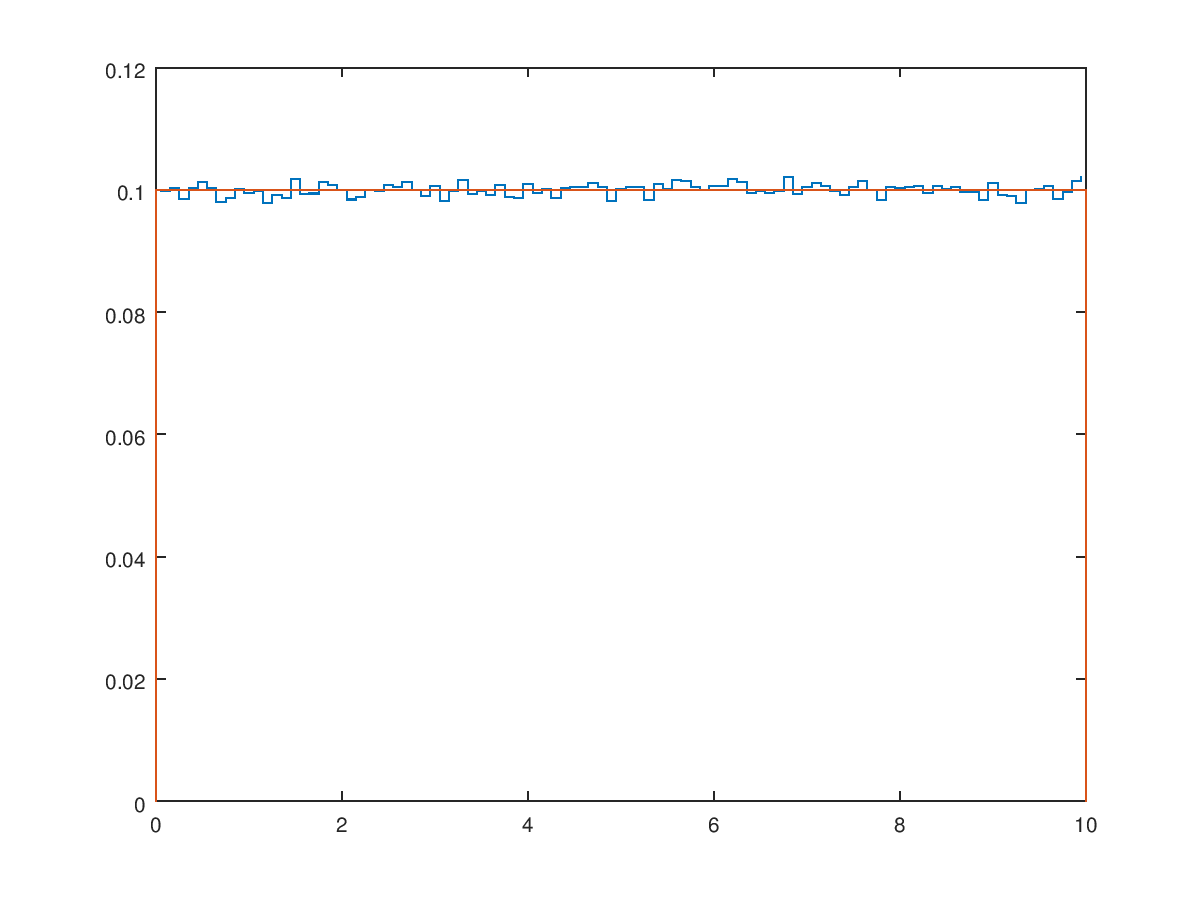
\includegraphics[width=\textwidth]{lab4_unif_plot.png}
		\caption{Равномерное}
	\end{minipage}\hfill
	\begin{minipage}{0.45\textwidth}
		\centering
		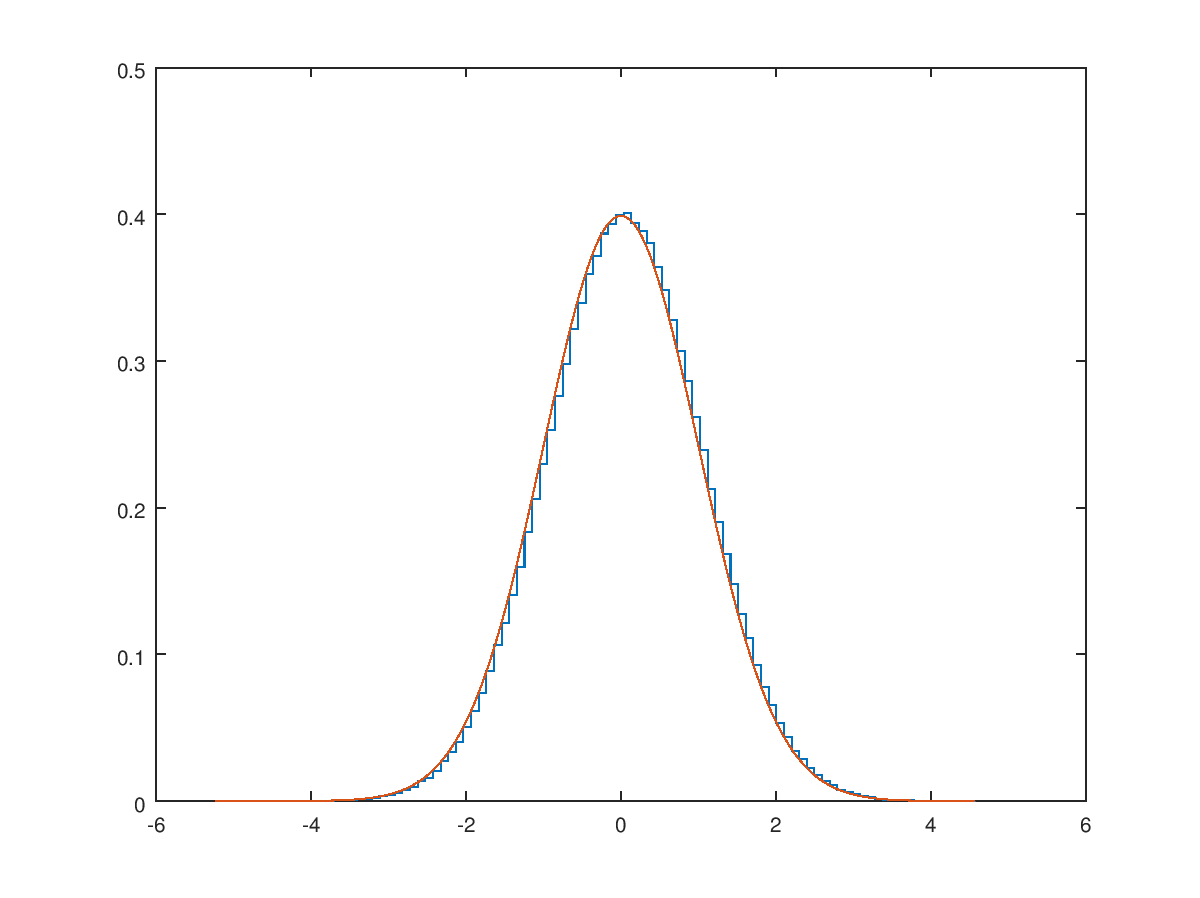
\includegraphics[width=\textwidth]{lab4_norm_plot.png}
		\caption{Нормальное}
	\end{minipage}
\end{figure}

\begin{itemize}
	\item Нормальное, код:
	\lstinputlisting[language=Octave]{lab4_norm_plot.m}
	
	\item Равномерное, код:
	\lstinputlisting[language=Octave]{lab4_unif_plot.m}
	
\end{itemize}

\begin{itemize}
	\item Нормальное
	\lstinputlisting[language=Octave]{t5.m}
	
	{\bf Выход:}
	
	\begin{lstlisting}
	Type I error alpha: 0.113000
	Type I error alpha (corrected): 0.072000
	Type II error beta with delta=0.005: 0.920000
	Type II error beta with delta=0.5: 0.000000\end{lstlisting}
	
	\item Равномерное
	\lstinputlisting[language=Octave]{t6.m}
	
	{\bf Выход:}
	
	\begin{lstlisting}
	Type I error alpha = 0.052000
	Type II error alpha with delta=0.005: 0.957000
	Type II error alpha with delta=0.5: 0.000000\end{lstlisting}
\end{itemize}

{\bf  Вывод:}

Построили гистограммы, получили эмпирическую оценку плотности. По графикам видно, что гистограмма достаточно хорошо приближает плотность.

Ошибки первого рода сходится с теоритическим значением по критерию хи-квадрат. Ошибка
второго рода реагирует только на сильные изменения, поэтому можно утверждать, что она
стремится к нулю при больших n.
\end{document}
